% **************************************************************************************************************
% A Classic Thesis Style
% An Homage to The Elements of Typographic Style
%
% Copyright (C) 2010 Andre Miede http://www.miede.de
%
% If you like the style then I would appreciate a postcard. My address 
% can be found in the file ClassicThesis.pdf. A collection of the
% postcards I received so far is available online at 
% http://postcards.miede.de
%
% License:
% This program is free software; you can redistribute it and/or modify
% it under the terms of the GNU General Public License as published by
% the Free Software Foundation; either version 2 of the License, or
% (at your option) any later version.
%
% This program is distributed in the hope that it will be useful,
% but WITHOUT ANY WARRANTY; without even the implied warranty of
% MERCHANTABILITY or FITNESS FOR A PARTICULAR PURPOSE.  See the
% GNU General Public License for more details.
%
% You should have received a copy of the GNU General Public License
% along with this program; see the file COPYING.  If not, write to
% the Free Software Foundation, Inc., 59 Temple Place - Suite 330,
% Boston, MA 02111-1307, USA.
%
% **************************************************************************************************************
% Note:
%    * You must not use "u etc. in strings/commands that will be spaced out (use \"u or real umlauts instead)
%    * New enumeration (small caps): \begin{aenumerate} \end{aenumerate}
%    * For margin notes: \graffito{}
%    * Do not use bold fonts in this style, it is designed around them
%    * Use tables as in the examples
%    * See classicthesis-ldpkg.sty for useful commands
% **************************************************************************************************************
% To Do:
%    * [high] Check this out: http://www.golatex.de/koma-script-warnung-in-verbindung-mit-listings-package-t2058.html
%    * [medium] mathbb in section-titles/chapter-titles => disappears somehow in headlines!!!
%    * [low] Calculate text block size for Libertine font
%    * [low] Think about processing a4paper, a5paper, 10pt, 11pt, 12pt etc. options for typearea layout
%            (store values in internal variables and handle by \AtEndOfPackage{\areaset...})
% **************************************************************************************************************
\documentclass[twoside=false,openright,titlepage,fleqn,numbers=noenddot,headinclude,%1headlines,% 
                11pt,a4paper,BCOR5mm,footinclude,cleardoublepage=empty,abstractoff % <--- obsolete, remove (todo)
                ]{scrreprt}

% ********************************************************************
% Development Stuff
% ********************************************************************
\listfiles
%\usepackage[l2tabu, orthodox, abort]{nag}
%\usepackage[warning, all]{onlyamsmath}
% ********************************************************************
% Re-usable information
% ********************************************************************
\newcommand{\myTitle}{SSHLauncher\xspace}
\newcommand{\myDegree}{Technical Report\xspace}
\newcommand{\myName}{Zdravko Bozakov\xspace}
\newcommand{\myProf}{Prof. Dr.-Ing. M. Fidler\xspace}
\newcommand{\myOtherProf}{Prof. Dr.-Ing. T. Kaiser\xspace}
\newcommand{\mySupervisor}{Dipl.-Ing. M. Bredel\xspace}
\newcommand{\myFaculty}{Fakult\"{a}t f\"{u}Elektrotechnik und Informationstechnik\xspace}
\newcommand{\myDepartment}{Institut f\"{u}r Kommunikationstechnik\xspace}
\newcommand{\myUni}{\protect{Leibniz Universit\"{a}}t Hannover\xspace}
\newcommand{\myLocation}{Hannover\xspace}
\newcommand{\myTime}{01. Mai 2009\xspace}
\newcommand{\myBirthdate}{01.Januar. 1970\xspace}
\newcommand{\myBirthplace}{Linuxhausen\xspace}
\newcommand{\myVersion}{Version 2.6.1\xspace}
% ********************************************************************
% Packages with options that might require adjustments
% ********************************************************************
\usepackage[latin1]{inputenc} 
\usepackage[ngerman,american]{babel}           
\usepackage[square,numbers]{natbib} 
\usepackage[fleqn]{amsmath} % math environments and more by the AMS 
\usepackage{float} % for H placement specifier
% ********************************************************************
\usepackage{classicthesis-ldpkg} 
% ********************************************************************
% Options for classicthesis.sty:
% tocaligned eulerchapternumbers drafting linedheaders listsseparated 
% subfig nochapters beramono eulermath parts minionpro pdfspacing 
% listings dottedtoc minionprospacing manychapters
\usepackage[eulerchapternumbers,drafting,listings,%pdfspacing,%
            subfig,beramono,eulermath,parts,dottedtoc]{classicthesis}

%*******************************************************
% Some font experiments
%*******************************************************
%\usepackage[osf]{libertine}
%\usepackage{hfoldsty}
%\usepackage[light,condensed,math]{iwona}
%\renewcommand{\sfdefault}{iwona}
%\usepackage{lmodern} % <-- no osf support :-(
%\usepackage[urw-garamond]{mathdesign} <-- no osf support :-(

% ********************************************************************  
% Fine-tuning for the text area
% ********************************************************************  
%\linespread{1.05} % a bit more for Palatino
%\areaset[5mm]{312pt}{761pt} % 686 (factor 2.2) + 33 head + 42 head \the\footskip
%\setlength{\marginparwidth}{7em}%
%\setlength{\marginparsep}{2em}%

% ********************************************************************  
% hack to use citations in float environments 
% will be fixed with caption package version 3.2
% ********************************************************************  
\usepackage{makerobust} 
\makeatletter 
%not working on OSX:
%\MakeRobustCommand\caption@xref 
\makeatother 

% ********************************************************************         
% Options for iktthesis.sty:
% abbrev exam big wiwi english
\usepackage[]{iktthesis}

\usepackage{fancyvrb}
% ********************************************************************
%\usepackage[section,below]{placeins} <--- not everybody wants this
%\usepackage[all]{hypcap} <--- does not work with MiKTeX 2.6
% ********************************************************************
% Language/strings for backrefs (change here, thanks, Lorenzo)
% ********************************************************************
%\renewcommand{\backrefnotcitedstring}{\relax}%(Not cited.)
%\renewcommand{\backrefcitedsinglestring}[1]{(Citato a pagina~#1.)}
%\renewcommand{\backrefcitedmultistring}[1]{(Citato alle pagine~#1.)}
%\renewcommand{\backreftwosep}{ e~}
%\renewcommand{\backreflastsep}{ e~}
% ********************************************************************
% Setup and Finetuning
% ********************************************************************
\newlength{\abcd} % for ab..z string length calculation
\newcommand{\myfloatalign}{\centering} % how all the floats will be aligned
\setlength{\extrarowheight}{3pt} % increase table row height
% ********************************************************************
% Captions look and feel
% ********************************************************************
\captionsetup{format=hang,font=small}
% ********************************************************************
% Listings setup
% ********************************************************************
%\lstset{emph={trueIndex,root},emphstyle=\color{BlueViolet}}%\underbar} % for special keywords
% ********************************************************************
\lstset{language=[LaTeX]Tex,%C++,
    keywordstyle=\color{RoyalBlue},%\bfseries,
    basicstyle=\small\ttfamily,
    %identifierstyle=\color{NavyBlue},
    commentstyle=\color{Green}\ttfamily,
    stringstyle=\rmfamily,
    numbers=none,%left,%
    numberstyle=\scriptsize,%\tiny
    stepnumber=5,
    numbersep=8pt,
    showstringspaces=false,
    breaklines=true,
    frameround=ftff,
    frame=single,
    belowcaptionskip=.75\baselineskip,
    numberbychapter=false
    %frame=L
} 

% ********************************************************************
% Where to look for graphics
% ********************************************************************
%\graphicspath{{gfx/}{misc/}} % considered harmful according to l2tabu
% ********************************************************************
% Hyperreferences
% ********************************************************************
\hypersetup{%
    colorlinks=true, linktocpage=true, pdfstartpage=3, pdfstartview=FitV,%
    % uncomment the following line if you want to have black links (e.g., for printing)
    %colorlinks=false, linktocpage=false, pdfborder={0 0 0}, pdfstartpage=3, pdfstartview=FitV,% 
    breaklinks=true, pdfpagemode=UseNone, pageanchor=true, pdfpagemode=UseOutlines,%
    plainpages=false, bookmarksnumbered, bookmarksopen=true, bookmarksopenlevel=1,%
    hypertexnames=true, pdfhighlight=/O,%hyperfootnotes=true,%nesting=true,%frenchlinks,%
    urlcolor=webbrown, linkcolor=RoyalBlue, citecolor=webgreen, %pagecolor=RoyalBlue,%
    % uncomment the following line if you want to have black links (e.g., for printing)
    %urlcolor=Black, linkcolor=Black, citecolor=Black, %pagecolor=Black,%
    pdftitle={\myTitle},%
    pdfauthor={\textcopyright\ \myName, \myUni, \myFaculty},%
    pdfsubject={},%
    pdfkeywords={},%
    pdfcreator={pdfLaTeX},%
    pdfproducer={LaTeX with hyperref and classicthesis}%
}
% ********************************************************************
% Hyphenation
% ********************************************************************
%\hyphenation{put special hyphenation here}
% ********************************************************************
% GO!GO!GO! MOVE IT!
% ********************************************************************
\begin{document}
\frenchspacing
\raggedbottom
\selectlanguage{american} % american ngerman
%\renewcommand*{\bibname}{new name}
%\setbibpreamble{}
\pagenumbering{roman}
\pagestyle{plain}
% ********************************************************************
% Frontmatter
% ********************************************************************

%*******************************************************
% Titlepage
%*******************************************************
%%%
%%% title page (german)
%%%
\pdfbookmark[0]{Titel Page}{title}
\begin{titlepage}
  \changetext{}{19mm}{}{19mm}{}
  \vspace{1cm}
  \begin{center}
    \includegraphics[width=13.8cm]{img/welfenschloss} \\ 
  \end{center}
  \medskip
  \begin{center}
    \textbf{\huge\spacedallcaps{L}\LARGE\spacedallcaps{eibniz}}
    \textbf{\huge\spacedallcaps{U}\LARGE\spacedallcaps{niversit\"{a}t}}
    \textbf{\huge\spacedallcaps{H}\LARGE\spacedallcaps{annover}} \\
  \end{center}

  \begin{center}
    \normalsize
    \spacedallcaps{Fakult\"{a}t}
    \spacedallcaps{f\"{u}r}
    \spacedallcaps{Elektrotechnik}
    \spacedallcaps{und}
    \spacedallcaps{Informatik} \\
    \smallskip
    \spacedallcaps{Institut}
    \spacedallcaps{f\"{u}r}
    \spacedallcaps{Kommunikationstechnik}
  \end{center}
  \vfill
  \vfill


  %*******************************************************
  % Titlepage for everyone else 
  %*******************************************************
  \begin{center}
    \LARGE \myTitle
  \end{center} 
  \vfill
  \vfill

  \begin{center}
    \LARGE \textbf{\myDegree}
  \end{center}
  \vfill

  \begin{center}
    %\large eingereicht von \\
  \end{center}

  \begin{center}
    \large \spacedallcaps{\myName}
  \end{center}

  \begin{center}
    \large \myTime \\
  \end{center} 
  \vfill

  \begin{center}
    \begin{tabular}{lll}
      %Erstpr\"{u}fer  & : & \myProf \\
      %Zweitpr\"{u}fer & : & \myOtherProf \\
      %Betreuer        & : & \mySupervisor
    \end{tabular}
  \end{center} 


%  \vfill

%  \begin{center}
%    \large \selectedthesisnumber \\
%  \end{center}

  \changetext{}{-19mm}{}{-19mm}{}

\end{titlepage}

\pagestyle{scrheadings}

%*******************************************************
% Table of Contents
%*******************************************************
%\phantomsection
\refstepcounter{dummy}
\pdfbookmark[1]{\contentsname}{tableofcontents}
\setcounter{tocdepth}{2} % <-- 2 includes up to subsections in the ToC
\setcounter{secnumdepth}{3} % <-- 3 numbers up to subsubsections
\manualmark
\markboth{\spacedlowsmallcaps{\contentsname}}{\spacedlowsmallcaps{\contentsname}}
\tableofcontents 

% ********************************************************************
% Mainmatter
% ********************************************************************
\pagenumbering{arabic}
% use \cleardoublepage here to avoid problems with pdfbookmark
% insert your chapters here
%\cleardoublepage\part{SSHLauncher}


\chapter{SSHLauncher Overview}
Simulation is a widely used paradigm for verifying existing theories
as well as novel approaches in communication networks. In order to
ensure the validity and credibility of simulation results, it is
crucial that sufficiently large numbers of simulation runs are
performed and statistics and corresponding confidence intervals are
presented. Unfortunately, the generation of sufficiently large amounts
of data can often be painstaking. In fact, the widespread credibility
problem of simulation studies has been analyzed in \cite{978060} and
\cite{1096174}.

Setups which rely on a number of different tools are typically
cumbersome to configure and difficult to automate. In cases where a
set of tools must be executed in a distributed environment, the task
of efficiently performing large numbers of experiments becomes even
more difficult.

Towards this end, the \emph{SSHLauncher} software aims to facilitate
the automated execution of experiments in distributed
environments. Moreover, the software allows users to execute large
sets of experiments and study the effects of parameter variation, with
minimal user intervention. The repetition of experiments becomes a
matter of executing a single command, allowing researchers to
concentrate on research tasks. In the course of our research we did
not find existing tools which adequately address these goals.


Each experiment is defined by a clear configuration script. As a side
effect, users are encouraged to generate documentation for their
work. Moreover, the experiment configuration file can be made
available to the community leading to easily reproducible
results. Faults in the experimental setup can be identified and
addressed more quickly. The importance of reproducible research has
been pointed out in \cite{schwab00, gentle07}.


\chapter{System Setup}

\emph{SSHLauncher} enables users to automate the execution of a set of commands on different hosts. A typical setup is depicted in Fig. \ref{fig:setup}. The hosts, corresponding commands and the dependencies which govern the execution order are specified in a configuration file stored on the control machine. As a result, after an initial configuration has been specified, complex experiments may be repeated an arbitrary number of times requiring almost no interaction from the user. The sole prerequisite is that all hosts allow remote SSH logins from the control machine. This is the case for almost all UNIX based operating systems and, using Cygwin, also under Windows. Additionally, a Python installation must be available on the control machine. Note that for experiments sensitive to network load it is advisable that separate data and control interfaces are present in the experiment setup, in order to minimize interference with ongoing measurements.

The Emulab \cite{Whiteosdi02} and PlanetLab \cite{956995} testbeds are examples of highly suitable environments for the use of \emph{SSHLauncher}.

\begin{figure}
  \centering
  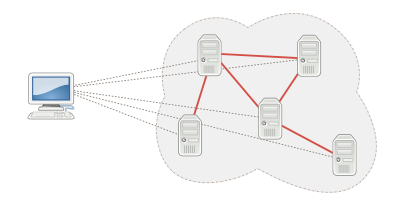
\includegraphics{img/setup_light}
  \caption{Typical SSHLauncher setup. Dashed lines represent
    control connections. }
  \label{fig:setup}
\end{figure}

\emph{SSHLauncher} utilizes the \emph{pexpect} and \emph{pxssh} Python modules written by Noah Spurrier \cite{pexpect}, which are also included in our distribution.

\chapter{Usage}

\section{Program Concept}
The idea behind \emph{SSHLauncher} is to automate the process of logging into remote hosts and executing a set of software tools. To achieve this the experiment commands are split into blocks and stored in a configuration file. Each configuration file block is associated with a specific SSH session. Similarly to the UNIX program \Verb=expect=, dependencies based on output strings of individual commands may be specified. In other words, each block of commands may contain numerous constraints as to when they can be executed. An analogy from project management are tasks in a Gantt chart, where certain tasks cannot begin before one or more other tasks have been completed.

The \emph{SSHLauncher} batch execution is initiated using the
following command:

\begin{verbatim}
$ sshlauncher [-d] CONFIGURATION
\end{verbatim}

where \Verb=<config>= is a mandatory configuration file containing a
series of hosts, commands and dependencies governing the execution
order. The configuration format will be described in detail in the
following chapters. The program establishes an SSH connection to all
hosts specified in the configuration file and executes the specified
commands, taking into account all given dependencies. As soon as the
execution of a specific configuration block is finished, i.e. the bash
prompt is reached on the destination host, the SSH session is
terminated. The \emph{SSHLauncher} terminates, when all configuration
blocks have been evaluated.

The optional parameter \Verb=-d= enables the debugging mode, causing \emph{SSHLauncher} to generate log-files containing the terminal output for every opened SSH connection. A log file is created for each configuration file section in the current working directory. Additionally, the program verbosity is increased.

\chapter{Configuration File Setup}

\section{Notation}
Throughout this document \Verb=<>= brackets will be used to denote an
arbitrary text string. Section tags not placed in brackets must be
written exactly as depicted. If not mentioned otherwise, square
brackets are to be treated as the literal characters \Verb=[= and
\Verb=]=.

The \emph{SSHLauncher} configuration file consists of a series of
so-called blocks or sections which specify the commands to be executed
on the destination host, as well as the order in which these are to be
run. The file format is based on the windows \emph{.INI} file
convention. Each section is identified by a unique section id and is
associated with a single SSH connection. The corresponding SSH session
is initiated when all block dependencies have been met, and is
terminated when all block commands have finished executing. The id tag
may contain any sequence of letters and digits and must be enclosed in
square brackets. The section id is followed by a number of parameters
identified by special tags. The tags include a user-name, destination
host name and the commands to be executed. Furthermore, a password can
be specified if SSH key authentication is not configured. The format
for a configuration file section is as follows:

\begin{Verbatim}
# <comment>
[<id>] 
user: <name>
password: <password>
host: <hostname>
command: <bash_commands>
\end{Verbatim}

The section tags are case-sensitive however, their order is not
relevant. Moreover, the order of the file sections may also be
arbitrary and does not effect the execution order. The number of
sections in a configuration file is only limited by the maximum number
of active SSH connections allowed by the system. Lines beginning with
\Verb=#= are treated as comments.

In addition to the tags described above, sections may contain the
\emph{after} tag. This tag implies, that the current section command
should only be executed after a specific string has been issued by a
command of another section. It is possible to include several
id/string pairs, separated by commas. In this case the section command
is executed after all strings have been matched. The \emph{after} tag
uses the python language dictionary notation:

\begin{Verbatim}
after: {'<id1>':'<string1>', ... ,'<idN>':'<stringN>'}
\end{Verbatim}

\section{Defaults and Variables}

In addition to the sections described above, which are always
associated with an SSH connection, a special \emph{default} section
can be specified in the configuration file. This section contains
default tag/value pairs which are appended to all other section in the
file. Tags also defined in a section override tags specified in the
default section. Furthermore, it is possible to define variables which
are accessible from within the sections. The format of the default
section is described below:

\begin{Verbatim}
[DEFAULT]
<varname1> = <value1>
<varname2> = <value2>
#
user: <name>
password: <password>
\end{Verbatim}

Variables can be useful as a shorthand for frequently used pathnames
or log filenames. To substitute a variable into any other part of the
configuration file formatted as a string the following notation must
be used: \Verb=%(<varname>)s=. For more details on variable usage,
please
refer to the examples chapter \ref{sec:example} of this document.

\section{External Variables}

It is possible to define special variables in the Bash shell, which
are imported and substituted into the configuration file. This feature
can be useful when performing large numbers of experiments, where only
a few parameters change in every run. The Bash variables are declared
as usual, however their name must be prefixed with \Verb=SL_=.

A typical Bash script that invokes \emph{SSHLauncher} with a varying
parameter, in this case packets per second, is depicted below:

\VerbatimInput{start_spruce.sh}

In the example above the variables \Verb=SL_I= and \Verb=SL_PPS= are
available from within the configuration file \Verb=spruce.config= and
may be used as follows:

\begin{Verbatim}
...
command: ITGSend -a node4 -t 600000 -C 2040 -c %(SL_PPS)s -rp 8999
...
\end{Verbatim}

\chapter{Notes and Tips}
Within a configuration section, it is legal to concatenate several
Bash commands using standard Bash operators such as \Verb=;= or
\Verb=&&=. These commands are then executed sequentially using a
single SSH connection. On the other hand, execution speed can be
increased if commands are run in parallel using separate SSH
connections. In order to keep the number of simultaneously opened SSH
sessions to a minimum, a connection is only established when all
strings in the \emph{after} tag have been matched.


Certain programs do not produce any text output. If other SSH section
commands depend on the termination of such a program, the user can
manually generate a string after the program completes using the
\emph{echo} command. This works reliably using the Bash shell.

\begin{Verbatim}
command: <bash_command>; echo 'finished command'
\end{Verbatim}


For tools which do not have a built-in logging support, it is often
desirable to redirect the output to a file. At the same time the
program's output should be available to \emph{SSHLauncher} in order to
trigger the execution of other command blocks. The Unix command
\emph{tee} can be useful for these cases.

\begin{Verbatim}
command: %(bindir)s/iperf -s | tee -i -a
%(logdir)s/%(SL_I)s_iperf_rcv.log  
\end{Verbatim}

A common source of problems is that some programs pipe their output to
\emph{stderr}, making it difficult for \emph{SSHLauncher} to pick up
the output. To circumvent this, Bash I/O redirection may be used,
e.g. \Verb=2>&1= redirects \emph{stderr} output to \emph{stdout}.

\begin{Verbatim}
command: %(bindir)s/pathchirp_snd 2>&1 | tee -a -i %(logdir)s/snd.log
\end{Verbatim}

To avoid polluting the Bash history of the destination hosts, history
saving is disabled.

It should be noted that the user must take care to avoid circular
references in the configuration file, which would cause the scripts to
wait indefinitely.

% before the section commands begin executing,
% \emph{SSHLauncher} attempts to detect circular references in the
% config file, which would cause the scripts to wait
% indefinitely. Nevertheless, the user must take care to avoid such
% cases.

\chapter{Sample Configuration}
\label{sec:example}
In this section a configuration file from a real-world scenario will
be outlined. A simple dumbbell setup in Emulab will be used to start
two sender and two receiver instances of the rude/crude traffic
generator \cite{rude}. The topology is depicted in \ref{fig:topo}. The
first flow will be sent from node0 to node5 and the second one from
node1 to node4.

\begin{figure}
  \centering
  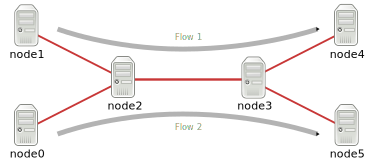
\includegraphics{img/topo_light}  
  \caption{Dumbell topology}
  \label{fig:topo}
\end{figure}

First we will define some default variables containing the tool
paths. Because the username is the same for all SSH connections it is
also included here. In our example SSH-key authentication is
configured, so there is no need to specify a password.

\begin{Verbatim}[fontsize=\footnotesize]
[DEFAULT]
log = /proj/Experiment/exp/results/active
bin  = /proj/Experiment/exp/wifi-simple/tools/rude_0.70/bin
home = /users/zbozakov

user: zbozakov
\end{Verbatim}

Next, we will do some cleaning up, i.e. remove all log files which
might have been left over from previous runs. As this section has no
\emph{after} tag, it will be executed right at the beginning. Note
that because the \Verb=rm= command usually does not produce any
output, a string is manually printed after the file deletion.

\begin{Verbatim}[fontsize=\footnotesize]
#### cleanup dirs ####
[cleanup]
host: node3.Dumbbell.Experiment.emulab.net
command: rm %(log)s/*bz2; rm %(log)s/*log; echo 'logs deleted'
\end{Verbatim}

In the next two sections the receivers are started on nodes 4 and
5. The \emph{after} tag ensures that the cleanup section has completed
before the connections are established. Moreover, we make use of the
variables defined in the default section.

\begin{Verbatim}[fontsize=\footnotesize]
### start receivers ####
## probe traffic receiver
[prcv]
host: node4.Dumbbell.Experiment.emulab.net
command: killall crude; %(bin)s/crude -P 1 -p 10001 -l
%(log)s/p_crude.bin.log
after: {'cleanup':'logs deleted'}
\end{Verbatim}

\begin{Verbatim}[fontsize=\footnotesize]
## cross traffic receiver
[xrcv]
host: node5.Dumbbell.Experiment.emulab.net
command: killall crude; %(bin)s/crude -P 1 -p 10001 -l
%(log)s/x_crude.bin.log
after: {'cleanup':'logs deleted'}
\end{Verbatim}

After the logs have been deleted and both receivers are running, the
senders can be started. Because the receiver (\emph{crude}) prints its
version information immediately after start up, we can use the string
\Verb='crude version'= for matching. To ensure that old instances of
the sender (\emph{rude}) will not interfere with the current run,
these are killed first. Both senders run for a predefined time and we
emit a string to signal that they are finished.

\begin{Verbatim}[fontsize=\footnotesize]
#### start senders ####
## probe traffic sender
[psnd]
host: node1.Dumbbell.Experiment.emulab.net
command: killall rude; %(bin)s/rude -s %(home)s/prb.cfg >
%(log)s/psnd.log; echo end
after: {'cleanup':'logs deleted', 'xrcv':'crude version',
'prcv':'crude version'}

## cross traffic sender
[xsnd]
host: node0.Dumbbell.Experiment.emulab.net
command: killall rude; %(bin)s/rude -s %(home)s/trc.cfg >
%(log)s/xsnd.log; echo end
after: {'cleanup':'logs deleted', 'xrcv':'crude version',
'prcv':'crude version'}
\end{Verbatim}

Finally, we include two more sections which kill the receivers and
compress the generated log files after both senders have terminated,
i.e. the string \Verb=end= has been issued by the senders.


\begin{Verbatim}[fontsize=\footnotesize]

#### terminate receivers and compress logs ####
## probe traffic receiver
[prcv_end]
host: node4.Dumbbell.Experiment.emulab.net
command: killall crude; bzip2 %(log)s/p*.log
after: {'psnd':'end'}

## cross traffic receiver
[xrcv_end]
host: node5.Dumbbell.Experiment.emulab.net
command: killall crude; bzip2 %(log)s/ar*.log
after: {'xsnd':'end'}
\end{Verbatim}


\chapter{Summary}

We presented \emph{SSHLauncher}, a tool which facilitates the
execution of multiple commands with dependencies in a distributed
environment. Using an intuitive configuration file syntax, large sets
of complex experiments can be performed with minimal user
interaction. \emph{SSHLauncher} was born out of necessity and was
heavily employed for generating data in \cite{BF08}. We hope that
other users will also find the software useful. 

The current version of the \emph{SSHLauncher} software together
with this documentation can be found at:
\url{http://www.ikt.uni-hannover.de/software.html}


\section*{Acknowledgements}
This work has been funded by an Emmy Noether grant of the German
Research Foundation.

\bibliographystyle{plainnat}
\bibliography{tr}

% ********************************************************************
% Game Over: Restart, Restore or Quit?
% ********************************************************************
\end{document}
% ********************************************************************
